\documentclass[natbib=true]{acmart}
\usepackage[utf8]{inputenc}
\usepackage[shortlabels]{enumitem}
\usepackage{subfig}
\usepackage{graphicx}
\usepackage{cleveref}
\usepackage{placeins}
\usepackage{colortbl}
\usepackage{bm}

\setcitestyle{numbers,sort&compress}

\title{Analysis of the stochastic spread of Stride simulation outcomes}

\author{Niels Aerens}
\author{Thomas Avé}
\author{Tobia De Koninck}
\author{Robin Jadoul}

\begin{abstract}
In this article we investigate a few properties of the Stride project. In particular we look at how to quantify the stochastic margins on the end result of a simulation run. Thereafter we try to identify how this information can be used for detecting unintended model changes with scenario tests.
\end{abstract}

\begin{document}

\maketitle

\section{Introduction}
Stride \cite{KUYLEN20172438} is an individual-based Simulator for the Transmission of Infectious Diseases with focus on model flexibility and
performance. 
Currently the Stride program has scenario tests to prevent regressions in the
simulation output. 
These tests use the Attack Rate as a parameter to assert the simulator outcome. Since Stride is a stochastic
system and thus relies on randomness, the output of its tests are variable.
The need for an acceptability range for the test outcome and the distribution of the test outcomes were examined.

\pagebreak

\section{Scenario tests}

The first test case of Stride (Influenza A \ref{sup:influenza_a}) performs a simulation of influenza in Flanders, with an $R_0$ \footnote{Basic reproduction number, a measure for the infectiousness of a disease: the amount of people 1 infected person will infect directly in a completely susceptible population.} value of 3.0.

The second test case (Influenza B) uses a seeding rate of 0, which results in a constant attack rate of 0. As expected, the RNG engine does not have influence on this outcome. 
The same holds for the third test case (Influenza C) which uses a very low seeding rate and a large immunity factor.
The attack vector for every run is 5.
The Measles 16 test case simulates the measles, the \(R_0\) value is set to 16, which results in a very large part of the population becoming infected. 
The last testcase (Measles 60) sets the $R_0$ value to 60. It infects the
whole population hence the attack rate is the same for all runs.

\section{Distribution of test outcome}

Before determining useful margins for the test outcome the distribution of these values has to be found.
The Stride program is using the TRNG library \citep{bauke2015tina} for generating random numbers. This libray is capable of using different RNG engines, therefore it is necessary to find the distribution of the attack rate for all these different random engines.
It is expected that all these random engines have the same distribution and that the outcomes are equivalent. 
The tested random number engines are \texttt{lgc64}, \texttt{lgc64\_shift}, \texttt{mrg2}, \texttt{mrg3}, \texttt{yarn2} and \texttt{yarn3}.

In order to do a statistical analysis, sufficient test data has to be generated. This was done using a Python script provided at \ref{sup:random_engines.py}. 
This script will execute stride 15 times for each random number engine, while choosing a seed for the number in the range \([0, 1000000000]\) using Python's \texttt{random.randint}\footnote{https://docs.python.org/3/library/random.html\#random.randint} method.
Python is using the \texttt{Mersenne Twister} as the core generator and generates a seed based on the random source of the operating system (e.g. \texttt{/dev/urandom} on a UNIX-like system) or the current time as a fallback.
Only the Influenza A and Measles 16 were tested since these are the only scenario tests without a constant Attack Rate. 
The script was adapated to generate 100 datapoints for each test case. The results can be found at \ref{sup:data-points:a} and \ref{sup:data-points:16} for respectively Influenza A and Measles 16.

A good starting point is testing whether it is normally distributed.
To give an estimate of the normality QQ-plots were used (see \cref{img:qq-plot:influenza_a} for an example). All QQ-plots can be found at \ref{sup:qq-plots}, histograms of the data can be found at \ref{sup:histograms}.
The QQ-plots already indicate rather normal distributed data. To formally confirm the normality the Shapiro-Wilk test was performed of which the p-values can be found in \cref{tab:influenza_a:shapiro} and \cref{tab:measles_16:shapiro}. 
All tests results in an (at least approximately) normal distribution for the attack rate.

\begin{figure}[!hbt]
    \centering
    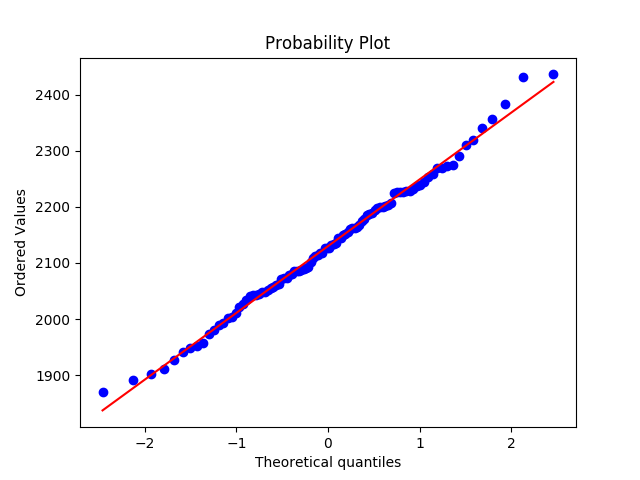
\includegraphics[width=0.7\textwidth]{images/influenza_a_qq_lgc64.png}
    \caption{QQ-Plot of Influenza A with the \texttt{lgc64} RNG engine}
    \label{img:qq-plot:influenza_a}
\end{figure}

\begin{table}[!hbt]
    \begin{tabular}{c c c c c c}
       \textbf{lgc64} & \textbf{lgc64\_shift} & \textbf{mrg2} & \textbf{mrg3} & \textbf{yarn2} & \textbf{yarn3}\\
        0.8719 & 0.4609 & 0.9385 & 0.6556 & 0.7254 & 0.7089
    \end{tabular}
    \caption{P-values of the Influenza A test case for the Shapiro-Wilk normality test}
    \label{tab:influenza_a:shapiro}
\end{table}

\begin{table}[!hbt]
    \begin{tabular}{c c c c c c}
       \textbf{lgc64} & \textbf{lgc64\_shift} & \textbf{mrg2} & \textbf{mrg3} & \textbf{yarn2} & \textbf{yarn3}\\
        0.8231 & 0.4216 & 0.9115 & 0.4199 & 0.1473 & 0.4431
    \end{tabular}
    \caption{P-values of the Measles 16 test case for the Shapiro-Wilk normality test}
    \label{tab:measles_16:shapiro}
\end{table}

\FloatBarrier

\section{Test Margins}

The scenario tests of Stride are run both sequential and parallel. 
OpenMP is used as library to facilitate the parallelization. 
As noted before Stride is a stochastic program and is using the TRNG library. 
The random number generation in stride is managed by the \texttt{RnManager} class, which ensures only one random number engine is constructed, because it is important not to generate the same random numbers (since only one seed is used during the simulator lifetime), which would be the behaviour when initialising RNG multiple times.

The parallelization of the test cases may cause differences in test outcome, even when using the same seed and RNG engine. 
Due to the unpredictable interleaving of the different threads, the random numbers generated will be drawn in a different order. 

In the sections that follow the different changes in the test environment and how they should be treated are discussed.

\subsection{When changing the implementation without altering the theoretical model}

The tests are using a constant seed, therefore one would expect that outcome of both the sequential and parallel tests do not change.

It may be the case that when refactoring or rewriting source code, the execution order of some parts changes.
As a result the usage of random numbers may change and therefore the test outcome changes although the theoretical and conceptual model have not changed. In other words, the implementation changed, but the underlying algorithms did not. 

Additionally the parallel tests will almost always vary in outcome for the reasons described earlier on.

It is clear that for the parallel tests there is no other option than working with a margin on the allowed outcomes.

There are a few options for the sequential tests. One of them is to have a constant outcome for this type of test.
The advantage is that a developer will be notified by the Continuous Integration service even for the slightest change in outcome. The developer can then validate this failure and check whether it is within the allowable margins and will re-calibrate or if the developer made a mistake in the code.

A second option is to have a margin for the sequential tests just like for the parallel tests. The developer will have less false-positive notifications of test failures.
On the other hand the chance that the developer has made a mistake that remains unnoticed is bigger. It may be preferred to use a smaller margin in this case.

A compromise could be to let the tests check if the outcome is the exact expected value. If this is the case the tests pass.
If not it checks if the outcome falls within the allowable margins. When this is the case only a warning is emitted but the tests pass. In all other cases the test fails.
This results in less false-positives, but the developer can't blindly trust the pass of a test. They have to check for warnings, which will be tough when using a CI system. % TODO: regular
This violates the principle of binary outcomes of software tests. 
Using a CI system with three states could solve this, but this may convert itself into a binary system again with only warning and failure.


Since it is known that the Attack Rate is normally distributed the standard deviation can be used to define a allowable margin.
It turns out that 2 times the standard deviation is a good fit since 95\% of the possible attack rates will fit between that range. 

\subsection{When changing the theoretical model}

This is the most challenging case. A change in the theoretical model should definitely be caught by the sequential tests (since these work without a margin), and ideally should be caught by the parallel tests too.
However since these do work with a margin it is possible that the change is too small to be out of the range.


When such a change is performed by the developer, a calibration tool should be used to calculate new values for both the sequential and parallel tests.
The developer of the change should be very cautious to blindly trust the calibration tool, and manually verify the new output of the tests.
In other words they should check if the change in outcome is what they expected when adapting the code.

\subsection{When changing the RNG engine}

Changing the RNG engine should not result in a ''big'' difference when using another engine. This difference can again be correctly qualified by using two times the standard deviation. 

Earlier on it was proven that independent of the choice of RNG engine the test outcome is normally distributed.
The same data and scripts were used to conclude that the different random number engines generate the same range of test outcomes.
Again only the Influenza A and Measles 16 were studied. The Levene test was used to test the equality of the standard deviation, a t-test for related samples was used for the means.

The hypotheses for the Levene test:
\[
\begin{aligned}
 H_0 &: \sigma_1 = \sigma_2\\
 H_1 &: \sigma_1 \ne \sigma_2\
\end{aligned}
\]

and for the t-test:
\[
\begin{aligned}
 H_0 &: \mu_1 = \mu_2  \\
 H_1 &: \mu_1 \ne \mu_2.
\end{aligned}
\]

The p-values for these tests are listed in \cref{tab:influenza:p_values} and \cref{tab:measles_16:p_values}. They clearly indicate that the \(H_0\) should not be rejected for both tests on a confidence level of $\alpha = 0.05$. Consequently, we can confidently conclude that the distribution of the attack rate does not differ significantly when using a different random engine.

\begin{table}[!hbt]
    \centering
    \bgroup
    \def\arraystretch{2}
    \begin{tabular}{c|c|c|c|c|c}
                                & \textbf{Influenza A}  & \textbf{Measles 16} \\ \hline
        \texttt{lgc64}          & \([1896, 2364]\)       & \([588959, 591317]\) \\
        \texttt{lgc64\_shift}   & \([1893, 2372]\)       & \([588992, 591360]\) \\
        \texttt{mrg2}           & \([1899, 2334]\)       & \([588967, 591307]\) \\
        \texttt{mrg3}           & \([1891, 2345]\)       & \([589012, 591268]\) \\
        \texttt{yarn2}          & \([1879, 2331]\)       & \([588836, 591615]\) \\
        \texttt{yarn3}          & \([1902, 2331]\)       & \([588751, 591443]\) \\
    \end{tabular}
    \egroup
    \caption{The acceptable attack rates for the Influenza A en Measles 16 test case for every random number engine}
    \label{tab:ranges_engines}
\end{table}

\begin{table}[!hbt]
    \centerline{\begin{tabular}{c|c|c|c|c|c|}
        & \textbf{lgc64} & \textbf{lgc64\_shift} & \textbf{mrg2} & \textbf{mrg3} & \textbf{yarn2} \\
        &  \( \bm{p_\mu} \quad \bm{p_\sigma} \)
            &  \( \bm{p_\mu} \quad \bm{p_\sigma} \)
            &  \( \bm{p_\mu} \quad \bm{p_\sigma} \)
            &  \( \bm{p_\mu} \quad \bm{p_\sigma} \)
            &  \( \bm{p_\mu} \quad \bm{p_\sigma} \) \\
        \textbf{lgc64\_shift}
            & \( 0.8819 \quad 0.7593 \)
            & \cellcolor{gray}
            & \cellcolor{gray}
            & \cellcolor{gray}
            & \cellcolor{gray} \\
        \textbf{mrg2}      
            & \( 0.2797 \quad 0.3763 \) 
            & \( 0.3359 \quad 0.2392 \) 
            & \cellcolor{gray}
            & \cellcolor{gray}
            & \cellcolor{gray} \\
        \textbf{mrg3}          
            & \( 0.3942 \quad 0.7113 \)
            & \( 0.3958 \quad 0.5026 \) 
            & \( 0.8842 \quad 0.6079 \) 
            & \cellcolor{gray}
            & \cellcolor{gray} \\
        \textbf{yarn2}        
            & \( 0.1507 \quad  0.5990 \)  
            & \( 0.1432 \quad 0.4116 \)  
            & \( 0.4590 \quad 0.7271 \) 
            & \( 0.4339 \quad 0.8737 \)  
            & \cellcolor{gray} \\
        \textbf{yarn3}          
            & \( 0.3578 \quad 0.4295 \)  
            & \( 0.3351 \quad 0.2750  \) 
            & \( 0.9843 \quad 0.9042  \)
            & \( 0.9017 \quad 0.6833 \) 
            & \( 0.4517 \quad 0.8102  \) \\
    \end{tabular}}
    \caption{P-values of the Influenza A test case}
    \label{tab:influenza:p_values}
\end{table}

\begin{table}[!hbt]
    \begin{tabular}{c|c|c|c|c|c|c}
        & \textbf{lgc64} & \textbf{lgc64\_shift} & \textbf{mrg2} & \textbf{mrg3} & \textbf{yarn2} \\
        &  \( \bm{p_\mu} \quad \bm{p_\sigma} \)
            &  \( \bm{p_\mu} \quad \bm{p_\sigma} \)
            &  \( \bm{p_\mu} \quad \bm{p_\sigma} \)
            &  \( \bm{p_\mu} \quad \bm{p_\sigma} \)
            &  \( \bm{p_\mu} \quad \bm{p_\sigma} \) \\
        \textbf{lgc64\_shift}
            & \( 0.2164 \quad 0.8855 \)
            & \cellcolor{gray}
            & \cellcolor{gray}
            & \cellcolor{gray}
            & \cellcolor{gray} \\
        \textbf{mrg2}      
            & \( 0.9754 \quad 0.8673 \) 
            & \( 0.2264 \quad 0.9838 \) 
            & \cellcolor{gray}
            & \cellcolor{gray}
            & \cellcolor{gray} \\
        \textbf{mrg3}          
            & \( 0.9630 \quad 0.9900 \)
            & \( 0.2671 \quad 0.8882 \) 
            & \( 0.9373 \quad 0.8687 \) 
            & \cellcolor{gray}
            & \cellcolor{gray} \\
        \textbf{yarn2}        
            & \( 0.3326 \quad 0.2670 \)  
            & \( 0.5949 \quad 0.2232 \)  
            & \( 0.3163 \quad 0.2107 \) 
            & \( 0.3081 \quad 0.2400 \)  
            & \cellcolor{gray} \\
        \textbf{yarn3}          
            & \( 0.6517 \quad 0.5366 \)  
            & \( 0.3611 \quad 0.4624 \) 
            & \( 0.6508 \quad 0.4457 \)
            & \( 0.6282 \quad 0.5097 \) 
            & \( 0.2195 \quad 0.6542 \) \\
    \end{tabular}
    \caption{P-values of the Measles 16 test case}
    \label{tab:measles_16:p_values}
\end{table}

\FloatBarrier

\subsection{When changing the seed for the RNG}

This is an extra test case added to the Stride test-suite to ensure that the seed provided by the random number engine doesn't change the test outcome.

Since a non-constant seed is used the sequential-test will not have a constant outcome anymore. Instead it will have the same margin as the parallel tests before (i.e. two times the standard deviation).

Again the same script was used to test for normality and thus the same output ranges was used as listed in \cref{tab:ranges_engines}.

\section{Supplementary Materials}

    \begin{enumerate}[label={[\arabic*]},ref={[sup~\arabic*]}]
        \item Influenza A scenario test \\
            \url{https://github.com/LEDfan/Bachelorproef/blob/master/test/cpp/gtester/ScenarioData.cpp\#L39}
            \label{sup:influenza_a}
    
        \item Python script to generate test data \\
            \url{https://ledfan.github.io/Bachelorproef/assets/src/paper-stochastisch/supplemental/random_engines.py} 
            \label{sup:random_engines.py}
            
        \item Data for Influenza A \\
            \url{https://ledfan.github.io/Bachelorproef/assets/src/paper-stochastisch/supplemental/engine_count_influenza.txt}
            \label{sup:data-points:a}
            
        \item Data for Measles 16 \\
            \url{https://ledfan.github.io/Bachelorproef/assets/src/paper-stochastisch/supplemental/engine_count_measles.txt}
            \label{sup:data-points:16}
            
        \item QQ-plots for Influenza A and Measles 16 for the different RNG engines \\ 
            \url{https://ledfan.github.io/Bachelorproef/assets/src/paper-stochastisch/supplemental/qq-plots.html} 
            \label{sup:qq-plots}
        
        \item Histograms for Influenza A and Measles 16 for the different RNG engines \\ 
            \url{https://ledfan.github.io/Bachelorproef/assets/src/paper-stochastisch/supplemental/histograms.html} 
            \label{sup:histograms}
            
    \end{enumerate}
    

\bibliographystyle{ACM-Reference-Format}
\bibliography{references.bib}

\end{document}

